%% This is an example first chapter.  You should put chapter/appendix that you
%% write into a separate file, and add a line \include{yourfilename} to
%% main.tex, where `yourfilename.tex' is the name of the chapter/appendix file.
%% You can process specific files by typing their names in at the 
%% \files=
%% prompt when you run the file main.tex through LaTeX.
\chapter{Introduction}\label{ch1:intro}
The pursuit of energy has shaped the history of mankind from its very beginning. And while the image of ancient humans huddled around fires for warmth, protection, and meal preparation is an archetype of our ancestral past, modern human needs remain much the same. Lighting to extend day into night, heating and cooling for residential comfort, cooking of the food we eat, access to the advanced technologies of our time --- these all require energy from one source or another. Choices abound, from animal and plant-based fuels, to buried hydrocarbon resources, to alternatives like solar, wind, hydro, nuclear, and geothermal. The balance and utilization of these resources can shape societal growth on the geopolitical stage and influence the very future of the habitable Earth.

This thesis examines how uncertainty characterization and risk mitigation can enhance the role of one source, geothermal, in addressing the ever-growing energy needs in a viable way. This chapter reflects on the extent of those needs and the conditions that may uniquely support an increased focus on geothermal as part of a commercial energy portfolio in the near-term. Opportunities and challenges associated with geothermal also lay the foundation for research questions motivating the remainder of this body of work.

\section{Energy Trends}\label{ch1:trends}
The \acrlong{eia} (\acrshort{eia}) publishes annual forecasts on U.S.\ energy generation and consumption in the \acrlong{aeo} (\acrshort{aeo}) report. Based on the 2020 reference case, the AEO model predicts a 70\% increase in U.S.\ energy usage by 2050, driven primarily by the industrial and power sectors \citep{eia_annual_2021}. Electricity generation also grows by a third, driven primarily by renewables and natural gas as coal, nuclear, and oil experience reductions (Figure \ref{fig:eia_2021_projections}). These predictions are offered with the caveat of much greater uncertainty due to the impact of the COVID-19 pandemic, although the EIA suggests a return to normal will occur by 2025 and broader, decadal trends will be unchanged \citep{eia_annual_2021}. International forecasts show similar growth in consumption and production, but traditional sources of energy like coal and natural gas also increase in capacity to meet the needs of India, China, and other rapidly developing nations \citep{eia_international_2020}. 
 
\begin{figure}[htp]
\centering
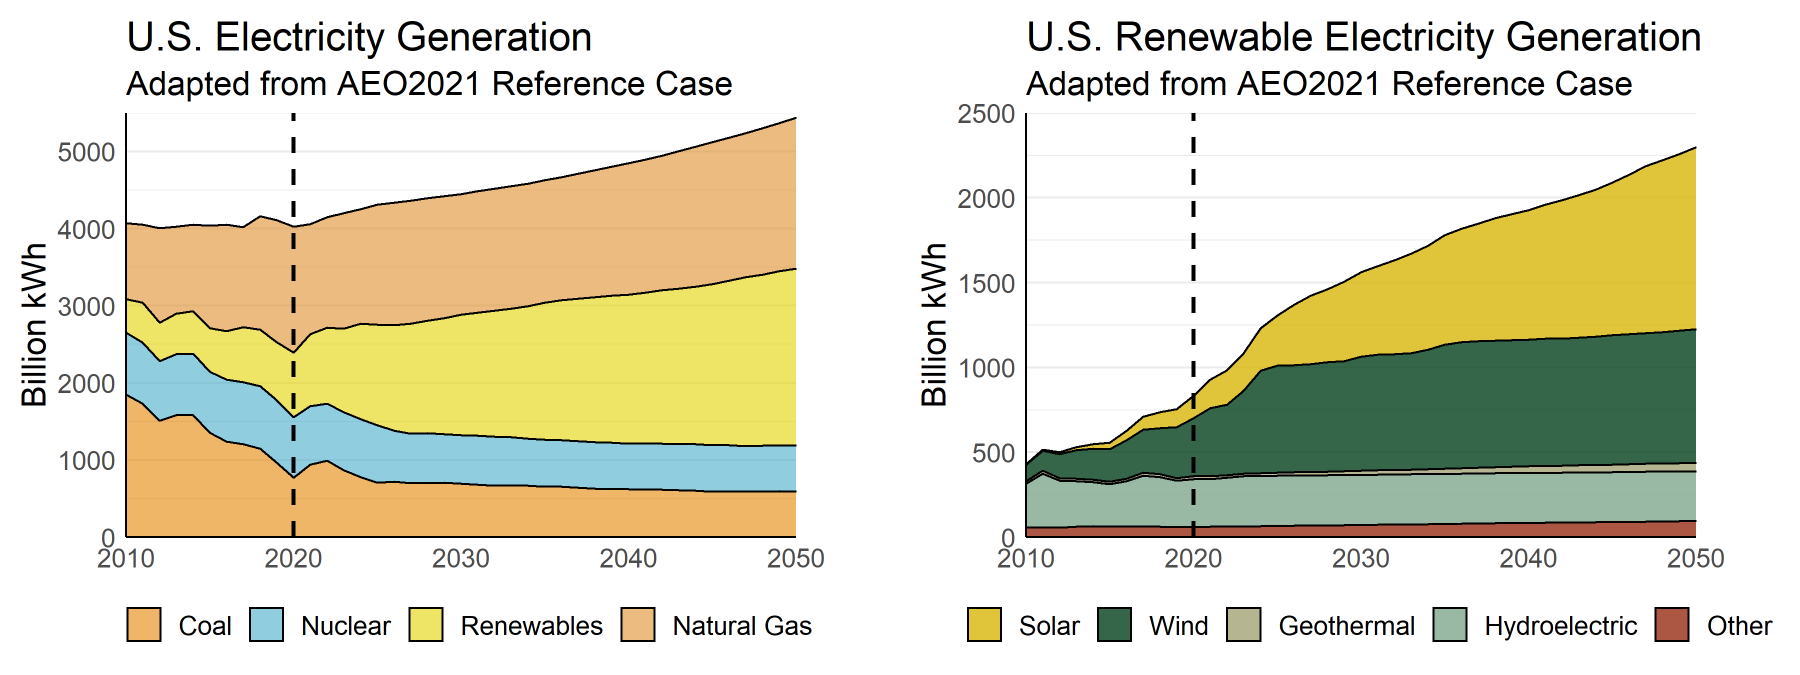
\includegraphics[width=\textwidth]{Figure-EIA_projections}
\caption[U.S.\ EIA projections based on the AEO2021 reference case]{U.S.\ EIA projections of (Left) U.S.\ electricity generation by fuel source and (Right) individual contributions by renewables based on the AEO2021 reference case \protect\citep{eia_annual_2021}. Vertical dashed line marks where historical records end and projections begin.}
\label{fig:eia_2021_projections}
\end{figure}

Lazard Asset Management breaks renewables down by \acrlong{lcoe} (\acrshort{lcoe}) in U.S.\ dollars/\acrshort{mwh}, where \acrshort{lcoe} is the estimated lifetime average net cost per unit energy of an electricity generating plant. In their 2020 analysis, intermittent energy sources like wind and utility-scale solar are already cost-competitive with fossil fuel-derived sources (Figure \ref{fig:lazard_lcoe}) \citep{lazard_lazards_2020}. Geothermal, an “always on” source of power, ranges from \$59-\$101/\acrshort{mwh} LCOE, making it second-tier in cost competitiveness but comparable to community and rooftop solar installations \citep{lazard_lazards_2020}. Overall, the transition in energy sources away from fossil fuel dominance is in progress, and the demand for energy in support of population growth and country development will remain a driver over the next 30 years.
 
\begin{figure}[htp]
\centering
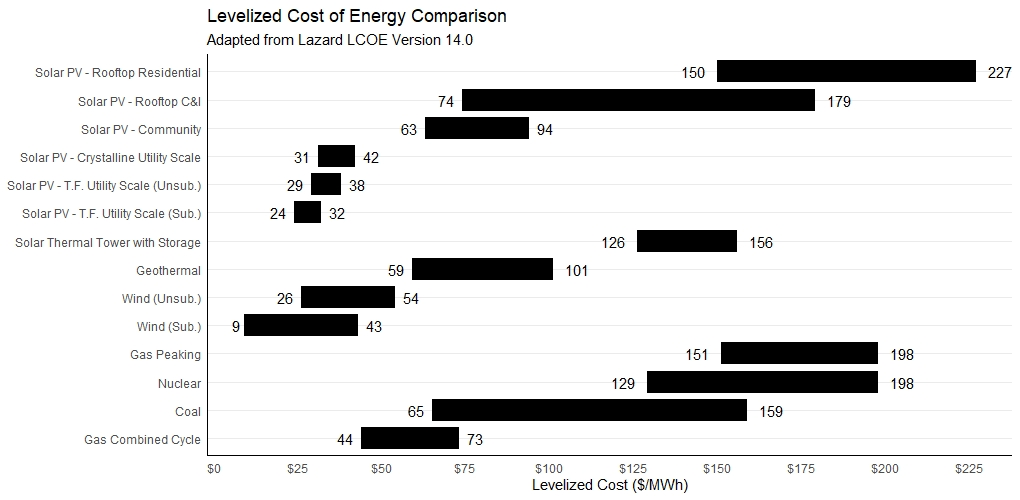
\includegraphics[width=\textwidth]{templates/images/Figure-Lazard_LCOE_recreated.jpeg}
\caption[Lazard Levelized Cost of Energy 2021 projections]{Cost comparison between different energy sources based on Lazard Asset Management LCOE analysis. C\&I: Commercial \& Industrial, T.F.: Thin Film, Unsub.: Unsubsidized, Sub.: Subsidized. For specific assumptions and caveats related to the analysis, see \protect\citet{lazard_lazards_2020}.}
\label{fig:lazard_lcoe}
\end{figure}

\section{Upstream Commercial Pressures}\label{ch1:upstream}
Businesses focused on \acrlong{ep} (\acrshort{ep}) of oil \& gas face a growing list of pressures influencing future corporate strategy. On one hand, the increase in energy consumption predicted in the AEO and IEO make the case for steadily ramping up production to provide plentiful supply to meet global demand; however, geopolitical tensions, state-ownership of oil companies, and breakthrough technologies create a volatile landscape unforgiving of an unsophisticated production approach. In just the past 15 years, major downturns in oil prices were triggered by a mixture of factors: the financial crisis, tied to banking practices and housing market instability in 2008 \citep{singh_2007-2008_2021}; increased production from U.S.\ unconventional plays and supply decisions from the \acrlong{opec} (\acrshort{opec}) in 2014 \citep{lioudis_what_2021}; and a price war between Russia and Saudi Arabia coinciding with a global pandemic in 2020 \citep{blessing_what_2021}. Additional uncertainty comes from national oil companies that control the majority of the world’s petroleum reserves, production, and rights for exploration and development. These state-run enterprises can eschew free-market principles, favoring national priorities over efficient operations, oil field sustainability, business transparency, and maximizing shareholder value \citep{pirog_role_2007}. Meanwhile, disruptive technologies like precise directional drilling and hydrofracturing have provided access to previously cost-prohibitive reserves, changing the balance of power as countries like the U.S.\ and China become less reliant on foreign hydrocarbon imports \citep{shuen_dynamic_2014}.

Layered on top of these strategic influences are the unexpected events that have enormous influence over energy production and distribution operations. The 2020 outbreak of the COVID-19 virus acted as an accelerator on longer-term trends of digital transformation and decarbonization in the oil \& gas industry. In the wake of a 25\% decrease in global demand, companies responded with massive layoffs and restructuring, a heightened focus on digitalization, and portfolio rationalizations that include shale write-downs and asset divestments \citep{deloitte_2021_2020}. Extreme weather events are shining a critical spotlight on how energy is managed now and in the future. Winter storm Uri blanketed Texas in record low temperatures in February 2021, shutting down liquid fuel supply and electricity generation from natural gas, coal, nuclear, and wind-based power plants, with downstream power blackouts, water outages, and surge pricing on electricity that impacted millions \citep{harc_winter_2021,lazard_lazards_2020}. And additional threats loom in the cyberworld as malicious hacking activities have rippling social and financial implications. One such attack on Colonial Pipeline, which handles almost 50\% of the liquid fuels supplied to the U.S.\ East Coast, led to gasoline shortages, price spikes, chemical factory shut-downs, and worldwide news coverage until the \$5 million ransom was paid in May 2021 \citep{sanger_pipeline_2021}.

\section{Net Zero Ambitions}\label{ch1:netzero}
The 2015 Paris climate agreement set a target of $<2^\circ$C on the rise in global temperatures above the pre-industrial average (i.e., the period from 1850-1900) to prevent the most extreme multiple-model predicted impacts of climate change \citep{unfccc_paris_2015}. The more commonly-ascribed $1.5^\circ$C target may be unachievable given current trajectories, and international calls to action are focusing on reducing anthropogenic carbon dioxide emissions to ``net zero'' as quickly as possible \citep{ipcc_global_2018}. Greater public awareness and discussion about these targets put pressure on the energy industry to revise their traditional business models. Beginning in 2020, top-tier oil and gas companies started issuing press releases outlining energy transition targets for 2025, 2030, 2050, and beyond \citep{bp_international_2020,chevron_chevron_2021,conocophillips_conocophillips_2020,equinor_equinor_2020,exxonmobil_exxonmobil_2021,shell_responsible_2020,shell_shell_2021,total_total_2020,total_2020_2021}. The proposed strategies vary but generally focus on (i) reducing company stake in fossil-fuel exploration and production activities, (ii) setting a net-zero target applicable to emissions from operations, product carbon intensity, and carbon offsets, and (iii) dedicating investments in low- and no-carbon energy alternatives to replace hydrocarbons. Nevertheless, pressure to do more, faster reached a new peak in May 2021 when a court decision in The Netherlands and shareholder votes for two U.S.\ majors demanded an accelerated push toward emissions reductions and low-carbon energy options \citep{mcwilliams_investors_2021}.

\section{Geothermal Energy}\label{ch1:geothermal}
Several factors must be met for an energy source to be considered a viable and sustainable alternative to the carbon-based fuels (coal, natural gas, oil) that currently meet much of the world’s energy needs.
\citet{glassley_geothermal_2015} notes a succinct set of criteria for such an energy resource: i) self-replenishment, ii) adequate abundance to meet energy demands, iii) low- to no-\acrlong{ghg} (\acrshort{ghg}) emissions, and iv) cost competitiveness compared to accessible alternatives. The first criterion distinctly defines renewable sources of energy like solar, gravitational, and geothermal. Solar energy includes both direct (sunlight) and indirect (wind, waves, water cycle) resources \citep{hohmeyer_ipcc_2008}. Gravitational energy drives the tides and supports energy-storage solutions like pumped-storage hydropower \citep{eere_pumped-storage_2021,hohmeyer_ipcc_2008}. And geothermal energy is primarily derived from the natural decay of radioactive isotopes within the Earth \citep{hohmeyer_ipcc_2008}. Table \ref{tab:renewableflux} specifically addresses criterion ii; the annual abundances of most renewable sources exceed energy demand, with geothermal scaling several orders of magnitude greater in annual flux/demand than other options \citep{hohmeyer_ipcc_2008}. Geothermal also meets the third criterion by providing a no-carbon source of energy that could support net zero aspirations when used in place of fossil fuels. The fourth criterion is less clear-cut. Geothermal costs depend strictly on use case, but as noted in Section \ref{ch1:trends}, LCOE analysis currently ranks geothermal third in the list of renewable options behind both wind and solar energy \citep{lazard_lazards_2020}. Does this make geothermal non-viable as an alternative? Perhaps no, as geothermal comes with several unique opportunities and benefits.

\begin{table}[h!]
\centering
\begin{tabular}{|l|l|l|}
\hline
\textbf{Renewable Source} & \textbf{Annual flux (EJ/yr)} & \textbf{Annual Flux/Demand*} \\ \hline
Solar      & 3,900,000   & 8,700  \\ \hline
Wind       & 6,000       & 13     \\ \hline
Hydro      & 149         & 0.33   \\ \hline
Bioenergy  & 2,900       & 6.5    \\ \hline
Ocean      & 7,400       & 17     \\ \hline
Geothermal & 140,000,000 & 31,000 \\ \hline
\end{tabular}
\caption[Annual renewable energy fluxes]{Annual renewable energy fluxes, based on Table 1 from \protect\citep{hohmeyer_ipcc_2008}. The ratio noted with * is based on global estimates from the same reference.}
\label{tab:renewableflux}
\end{table}

Most fundamentally, geothermal energy offers a reliable, nearly inexhaustible resource accessible anywhere around the world. Unlike wind and solar, which depend on favorable locations and vary with season and time of day, geothermal is both consistent and continuous. It could provide dependable baseload power for regional electrical grids without the additional need of assistive energy-storage technology \citep{tester_future_2006}. Based on history, one might assume geothermal only works under conventional conditions involving active hydrothermal circulation near volcanic zones (e.g., Iceland, Indonesia) or within major rift zones (e.g., East African Rift). However, additional opportunities lie in low-temperature direct-use geothermal for building heating and cooling, industrial processing, agricultural activities, and manufacturing \citep{glassley_geothermal_2015}. And technology supporting Enhanced Geothermal Systems (EGS) provides access to subsurface heat in areas without hydrothermal conditions \citep{tester_future_2006}. Natural radioactive decay takes place throughout the entirety of the Earth’s crust, contributing to the increasing temperature with depth profile known as the geotherm or geothermal gradient \citep{fowler_solid_2005}. Where there is a strong gradient, there is the potential for geothermal energy capture.

For all its benefits, the use of geothermal energy comes with its own unique set of challenges and risks. Many mirror the challenges faced by oil and gas producers, like issues related to drilling equipment and borehole integrity. For every well drilled, there is the risk of low resource quality, poor reservoir productivity, unexpected structural and stratigraphic complexity, and undesirable fluid chemistry \citep{beckers_low-temperature_2016, hadi_resource_2010}. Similarities between petroleum and geothermal development extend into unconventionals/EGS, where risks around hydrofracturing include inadequate permeable rock volume within the stimulated fracture zone, short-circuiting of fluid flow between injection and productions wells, fluid losses within the subsurface, and induced seismic activity \citep{jelacic_evaluation_2008,pan_establishment_2019}. As in oil \& gas projects, the former set of challenges could be mitigated by an appropriate level of subsurface characterization, and the latter would benefit from high-resolution reservoir and fracture modeling. Note that this overlap in challenges and required skill sets between oil \& gas and geothermal is unique among all renewable energy options. Skill and knowledge transfer between the two domains could directly benefit geothermal operations and risk mitigation strategies \citep{petty_synergies_2009}. And adding geothermal to the overall asset portfolio provides a simplified pathway for Upstream companies to meet net zero commitments while retaining and utilizing existing talent.

One of the most significant uncertainties for geothermal is cost. The scope of an LCOE assessment considers all costs in a geothermal project, from early exploration, through development drilling and power plant construction, to operations and maintenance over a 25- to 30-year lifetime \citep{beckers_introducing_2013, entingh_volume_2006, tester_economic_1990}. Studies show drilling of exploration, confirmation, injection, and production wells can account for 60-75\% of the total EGS project cost \citep{lukawski_uncertainty_2016, petty_synergies_2009}. New drilling technologies being developed may help address both cost uncertainty and potential value ranges \citep{nrel_2020_2020}. However, significant project savings could be achieved through better characterization prior to drilling the first exploration well; increasing the probability of well success without multi-million dollar well failures could bring down the overall LCOE. In addition, choices in the design of the geothermal power plant may also have significant cost implications over the life of a geothermal field. Lessons can be learned from power plants built against design specifications that prove unsupported by actual production conditions \citep{manente_hybrid_2011}. Improving the overall economics of geothermal could start with recognizing uncertainties in the system and using those uncertainties to make better decisions on \textit{where to drill} and \textit{how to build}. Providing the appropriate tools and methods to make these decisions will also help oil \& gas companies bridge the gap between traditional business strategies and lower-carbon energy production with geothermal as part of their energy mix.

\section{Research Questions}\label{ch1:researchqs}
Based on the aforementioned opportunity to integrate uncertainty characterization with geothermal exploration and development decision-making for petroleum companies, this thesis will address the following research questions:

\begin{itemize}
  \item Can geothermal exploration risk be mitigated using insights derived from readily-available data sources? And if gaps exist, can the data highlight additional actions for reducing risk before drilling a geothermal well?
  \item How can the recognition and characterization of present and future uncertainties influence the development strategy for geothermal facilities? In what ways will such an approach mitigate risk, if at all?
\end{itemize}

\section{Thesis Outline}\label{ch1:outline}

\begin{figure}[!htp]
\onehalfspacing
\begin{minipage}[b]{0.53\textwidth}
This thesis follows the flow shown in Figure \ref{fig:thesis_flow} and is structured as follows: 
\begin{itemize}
\item Chapter 2 provides relevant background on the origins of geothermal heat, types of geothermal systems, and a literature review on geothermal exploration and facility planning.
\item Chapters 3--4 explain the sources of data used in the thesis, data preparation strategies, and the chosen methods for predictive analytics (Ch.\ 3) and cost modeling of geothermal facility project designs (Ch.\ 4).
\item Chapters 5--6 describe and discuss the analytics results (Ch.\ 5) and cost modeling results (Ch.\ 6).
\item Chapter 7 frames learnings from the previous chapters as risk mitigation actions in a comprehensive geothermal business strategy.
\end{itemize}
\end{minipage} \hfill
\begin{minipage}[b]{0.44\textwidth}
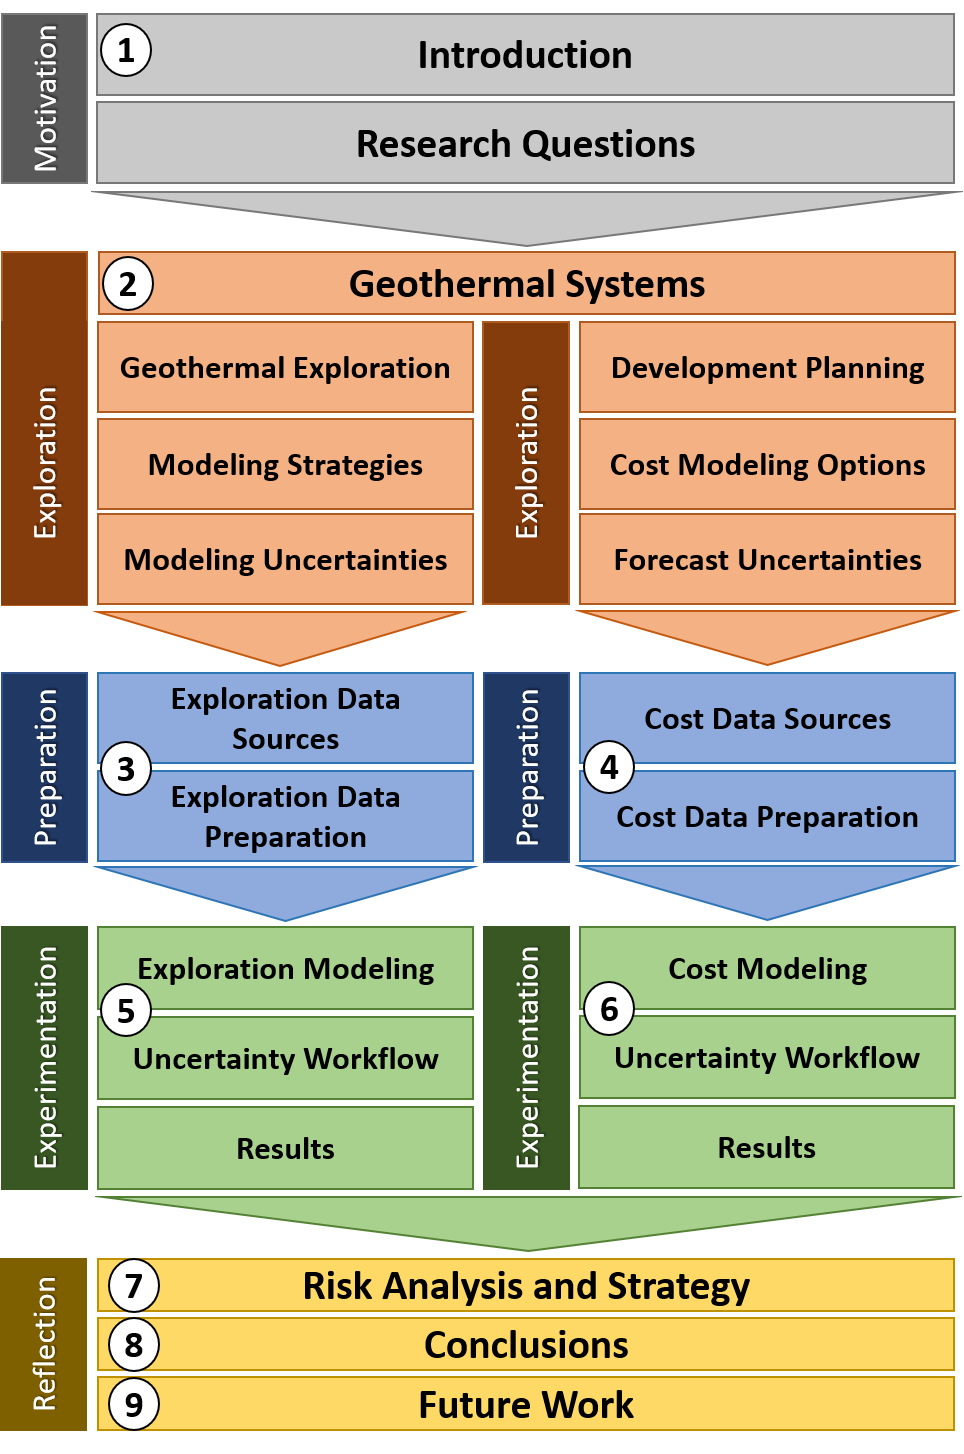
\includegraphics[scale=0.44]{Figure-ThesisWorkflow}
\caption[Flow chart for thesis structure]{Flow chart of thesis structure. Chapter numbers are circled.}
\label{fig:thesis_flow}
\end{minipage}
\begin{itemize}
\item Chapters 8 and 9 conclude the thesis with a summary of thesis insights (Ch.\ 8) and a list of future work opportunities (Ch.\ 9).
\end{itemize}
\end{figure}

%\begin{wrapfigure}[4in]{R}{0.5\linewidth}
%%\vspace{-10pt}
%%\centering
%%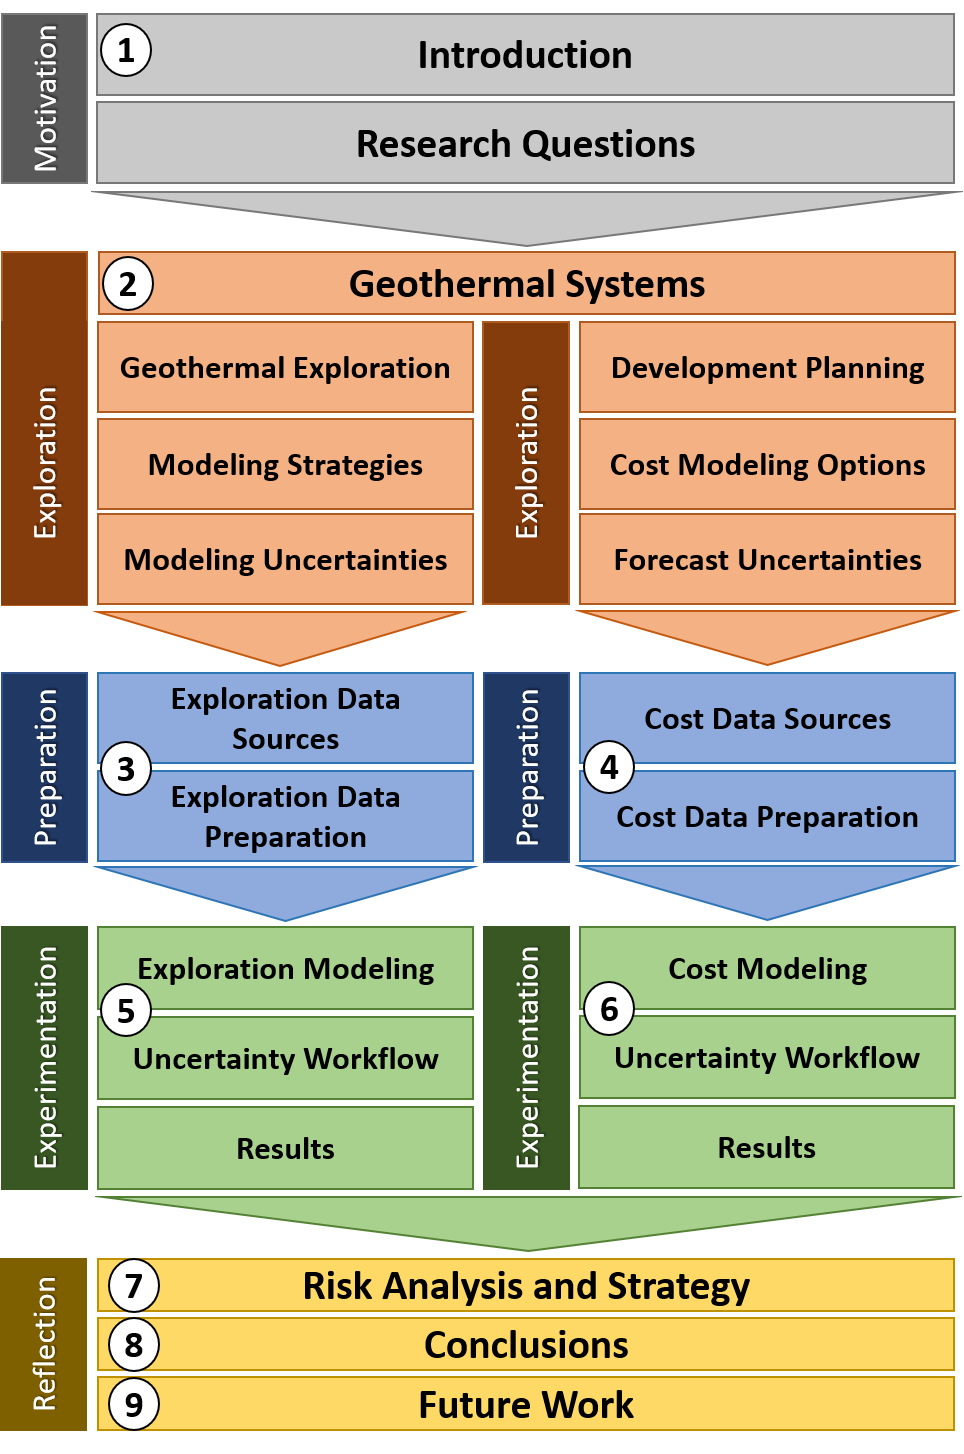
\includegraphics[scale=0.45]{Figure-ThesisWorkflow}
%%\caption[Flow chart for thesis structure]{Flow chart of thesis structure. Chapter number placement indicates the content presented within each chapter.} 
%%\label{fig:thesis_flow}
%%\end{wrapfigure}